\documentclass[twoside]{article}

% Packages required by doxygen
\usepackage{fixltx2e}
\usepackage{calc}
\usepackage{doxygen}
\usepackage[export]{adjustbox} % also loads graphicx
\usepackage{graphicx}
\usepackage[utf8]{inputenc}
\usepackage{makeidx}
\usepackage{multicol}
\usepackage{multirow}
\PassOptionsToPackage{warn}{textcomp}
\usepackage{textcomp}
\usepackage[nointegrals]{wasysym}
\usepackage[table]{xcolor}

% Font selection
\usepackage[T1]{fontenc}
\usepackage[scaled=.90]{helvet}
\usepackage{courier}
\usepackage{amssymb}
\usepackage{sectsty}
\renewcommand{\familydefault}{\sfdefault}
\allsectionsfont{%
  \fontseries{bc}\selectfont%
  \color{darkgray}%
}
\renewcommand{\DoxyLabelFont}{%
  \fontseries{bc}\selectfont%
  \color{darkgray}%
}
\newcommand{\+}{\discretionary{\mbox{\scriptsize$\hookleftarrow$}}{}{}}

% Page & text layout
\usepackage{geometry}
\geometry{%
  a4paper,%
  top=2.5cm,%
  bottom=2.5cm,%
  left=2.5cm,%
  right=2.5cm%
}
\tolerance=750
\hfuzz=15pt
\hbadness=750
\setlength{\emergencystretch}{15pt}
\setlength{\parindent}{0cm}
\setlength{\parskip}{3ex plus 2ex minus 2ex}
\makeatletter
\renewcommand{\paragraph}{%
  \@startsection{paragraph}{4}{0ex}{-1.0ex}{1.0ex}{%
    \normalfont\normalsize\bfseries\SS@parafont%
  }%
}
\renewcommand{\subparagraph}{%
  \@startsection{subparagraph}{5}{0ex}{-1.0ex}{1.0ex}{%
    \normalfont\normalsize\bfseries\SS@subparafont%
  }%
}
\makeatother

% Headers & footers
\usepackage{fancyhdr}
\pagestyle{fancyplain}
\fancyhead[LE]{\fancyplain{}{\bfseries\thepage}}
\fancyhead[CE]{\fancyplain{}{}}
\fancyhead[RE]{\fancyplain{}{\bfseries\leftmark}}
\fancyhead[LO]{\fancyplain{}{\bfseries\rightmark}}
\fancyhead[CO]{\fancyplain{}{}}
\fancyhead[RO]{\fancyplain{}{\bfseries\thepage}}
\fancyfoot[LE]{\fancyplain{}{}}
\fancyfoot[CE]{\fancyplain{}{}}
\fancyfoot[RE]{\fancyplain{}{\bfseries\scriptsize Generated by Doxygen }}
\fancyfoot[LO]{\fancyplain{}{\bfseries\scriptsize Generated by Doxygen }}
\fancyfoot[CO]{\fancyplain{}{}}
\fancyfoot[RO]{\fancyplain{}{}}
\renewcommand{\footrulewidth}{0.4pt}
\renewcommand{\sectionmark}[1]{%
  \markright{\thesection\ #1}%
}

% Indices & bibliography
\usepackage{natbib}
\usepackage[titles]{tocloft}
\setcounter{tocdepth}{3}
\setcounter{secnumdepth}{5}
\makeindex

% Hyperlinks (required, but should be loaded last)
\usepackage{ifpdf}
\ifpdf
  \usepackage[pdftex,pagebackref=true]{hyperref}
\else
  \usepackage[ps2pdf,pagebackref=true]{hyperref}
\fi
\hypersetup{%
  colorlinks=true,%
  linkcolor=blue,%
  citecolor=blue,%
  unicode%
}

% Custom commands
\newcommand{\clearemptydoublepage}{%
  \newpage{\pagestyle{empty}\cleardoublepage}%
}

\usepackage{caption}
\captionsetup{labelsep=space,justification=centering,font={bf},singlelinecheck=off,skip=4pt,position=top}

%===== C O N T E N T S =====

\begin{document}

% Titlepage & ToC
\hypersetup{pageanchor=false,
             bookmarksnumbered=true,
             pdfencoding=unicode
            }
\pagenumbering{alph}
\begin{titlepage}
\vspace*{7cm}
\begin{center}%
{\Large /home/bblaskova/\+Net\+Beans\+Projects/\+I\+V\+S-\/\+New-\/\+Meta }\\
\vspace*{1cm}
{\large Generated by Doxygen 1.8.13}\\
\end{center}
\end{titlepage}
\pagenumbering{roman}
\tableofcontents
\pagenumbering{arabic}
\hypersetup{pageanchor=true}

%--- Begin generated contents ---
\section{I\+V\+S-\/\+New-\/\+Meta}
\label{md_README}
\Hypertarget{md_README}
\subsubsection*{Prostredi }

Ubuntu 32bit Ubuntu 64bit Windows 32bit Windows 64bit

\subsubsection*{Autori }

Nazev tymu
\begin{DoxyItemize}
\item xblask04 Barbora Blašková
\item xcrkon00 Jakub Crkoň
\item xkosti05 Gabriel Koštialik
\end{DoxyItemize}

\subsubsection*{Licence }

G\+NU G\+E\+N\+E\+R\+AL P\+U\+B\+L\+IC L\+I\+C\+E\+N\+SE Version 3, 29 June 2007 
\section{Hierarchical Index}
\subsection{Class Hierarchy}
This inheritance list is sorted roughly, but not completely, alphabetically\+:\begin{DoxyCompactList}
\item \contentsline{section}{math}{\pageref{classmath}}{}
\item \contentsline{section}{math\+Test}{\pageref{classmathTest}}{}
\item Application\begin{DoxyCompactList}
\item \contentsline{section}{Calculator}{\pageref{classCalculator}}{}
\end{DoxyCompactList}
\item Initializable\begin{DoxyCompactList}
\item \contentsline{section}{Credits\+Controller}{\pageref{classCreditsController}}{}
\item \contentsline{section}{G\+U\+I\+\_\+\+Controller}{\pageref{classGUI__Controller}}{}
\item \contentsline{section}{Help\+\_\+controller}{\pageref{classHelp__controller}}{}
\end{DoxyCompactList}
\end{DoxyCompactList}

\section{Class Index}
\subsection{Class List}
Here are the classes, structs, unions and interfaces with brief descriptions\+:\begin{DoxyCompactList}
\item\contentsline{section}{\hyperlink{classCalculator}{Calculator} }{\pageref{classCalculator}}{}
\item\contentsline{section}{\hyperlink{classCreditsController}{Credits\+Controller} }{\pageref{classCreditsController}}{}
\item\contentsline{section}{\hyperlink{classGUI__Controller}{G\+U\+I\+\_\+\+Controller} }{\pageref{classGUI__Controller}}{}
\item\contentsline{section}{\hyperlink{classHelp__controller}{Help\+\_\+controller} }{\pageref{classHelp__controller}}{}
\item\contentsline{section}{\hyperlink{classmath}{math} }{\pageref{classmath}}{}
\item\contentsline{section}{\hyperlink{classmathTest}{math\+Test} }{\pageref{classmathTest}}{}
\end{DoxyCompactList}

\section{File Index}
\subsection{File List}
Here is a list of all documented files with brief descriptions\+:\begin{DoxyCompactList}
\item\contentsline{section}{src/\hyperlink{Calculator_8java}{Calculator.\+java} \\*Main class -\/ \hyperlink{classCalculator}{Calculator} }{\pageref{Calculator_8java}}{}
\item\contentsline{section}{src/\hyperlink{GUI__Controller_8java}{G\+U\+I\+\_\+\+Controller.\+java} \\*Contains button actions }{\pageref{GUI__Controller_8java}}{}
\item\contentsline{section}{src/\hyperlink{math_8java}{math.\+java} \\*Class with mathematic operation used in calculator }{\pageref{math_8java}}{}
\item\contentsline{section}{test/\hyperlink{mathTest_8java}{math\+Test.\+java} \\*Tests for \hyperlink{math_8java}{math.\+java} library }{\pageref{mathTest_8java}}{}
\end{DoxyCompactList}

\section{Class Documentation}
\hypertarget{classCalculator}{}\subsection{Calculator Class Reference}
\label{classCalculator}\index{Calculator@{Calculator}}
Inheritance diagram for Calculator\+:\begin{figure}[H]
\begin{center}
\leavevmode
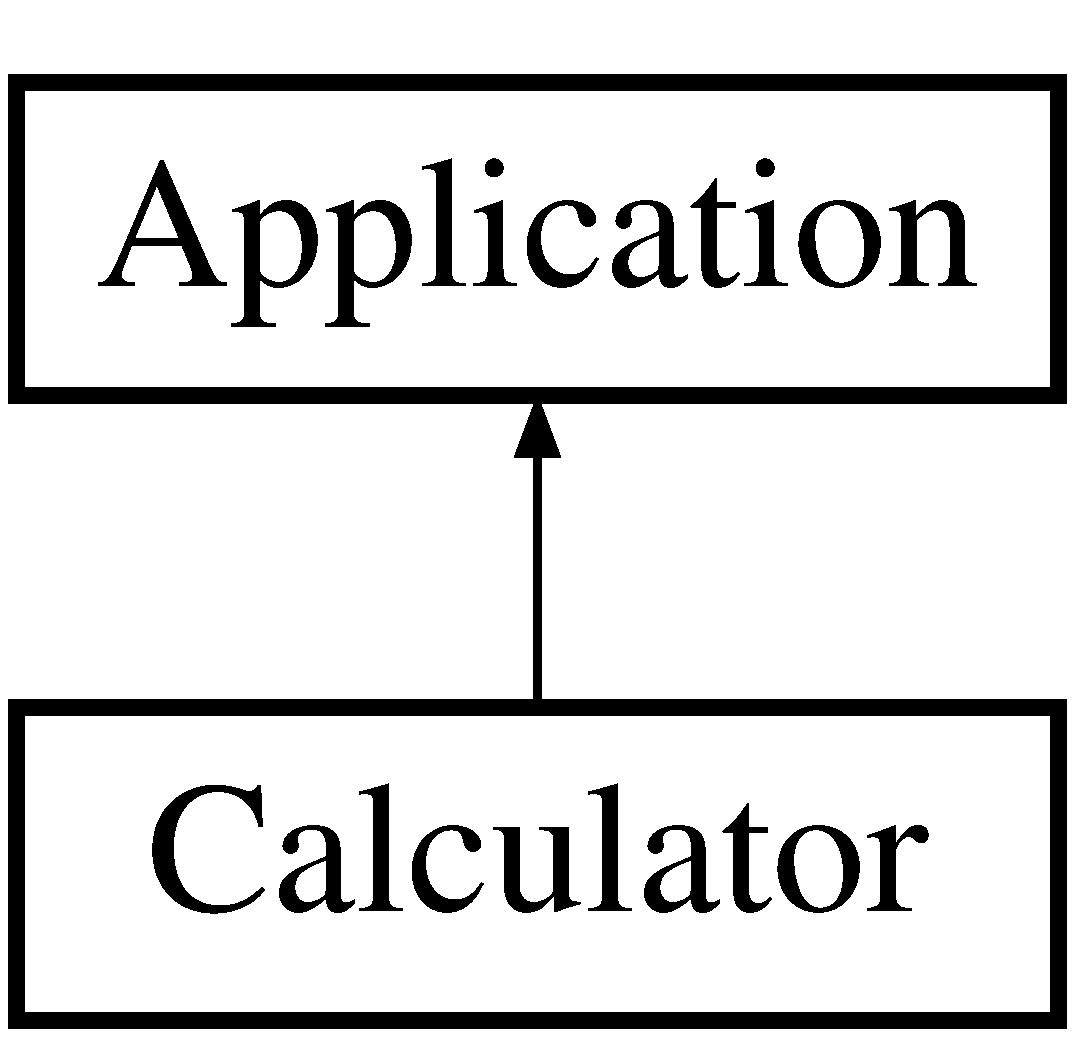
\includegraphics[height=2.000000cm]{classCalculator}
\end{center}
\end{figure}
\subsubsection*{Public Member Functions}
\begin{DoxyCompactItemize}
\item 
\mbox{\Hypertarget{classCalculator_a4aa738e7d39fe99e500fbb0778ca5046}\label{classCalculator_a4aa738e7d39fe99e500fbb0778ca5046}} 
void {\bfseries start} (Stage stage)  throws Exception 
\end{DoxyCompactItemize}
\subsubsection*{Static Public Member Functions}
\begin{DoxyCompactItemize}
\item 
static void \hyperlink{classCalculator_a1efab50ed4696158d68289e20c255e7f}{main} (String\mbox{[}$\,$\mbox{]} args)
\begin{DoxyCompactList}\small\item\em Main function of the calculator. \end{DoxyCompactList}\end{DoxyCompactItemize}


\subsubsection{Member Function Documentation}
\mbox{\Hypertarget{classCalculator_a1efab50ed4696158d68289e20c255e7f}\label{classCalculator_a1efab50ed4696158d68289e20c255e7f}} 
\index{Calculator@{Calculator}!main@{main}}
\index{main@{main}!Calculator@{Calculator}}
\paragraph{\texorpdfstring{main()}{main()}}
{\footnotesize\ttfamily static void Calculator.\+main (\begin{DoxyParamCaption}\item[{String \mbox{[}$\,$\mbox{]}}]{args }\end{DoxyParamCaption})\hspace{0.3cm}{\ttfamily [inline]}, {\ttfamily [static]}}



Main function of the calculator. 


\begin{DoxyParams}{Parameters}
{\em args} & the command line arguments \\
\hline
\end{DoxyParams}


The documentation for this class was generated from the following file\+:\begin{DoxyCompactItemize}
\item 
src/\hyperlink{Calculator_8java}{Calculator.\+java}\end{DoxyCompactItemize}

\hypertarget{classCreditsController}{}\subsection{Credits\+Controller Class Reference}
\label{classCreditsController}\index{Credits\+Controller@{Credits\+Controller}}
Inheritance diagram for Credits\+Controller\+:\begin{figure}[H]
\begin{center}
\leavevmode
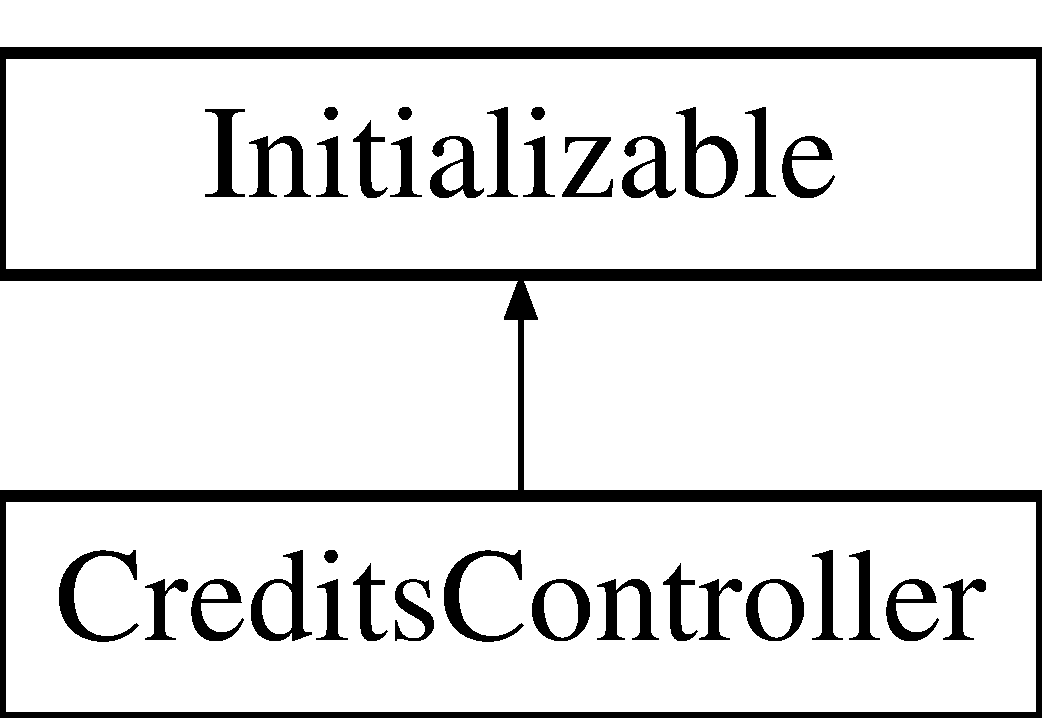
\includegraphics[height=2.000000cm]{classCreditsController}
\end{center}
\end{figure}
\subsubsection*{Public Member Functions}
\begin{DoxyCompactItemize}
\item 
void \hyperlink{classCreditsController_a30a25651d36cbea8bd963e42a908696b}{initialize} (U\+RL url, Resource\+Bundle rb)
\end{DoxyCompactItemize}
\subsubsection*{Private Member Functions}
\begin{DoxyCompactItemize}
\item 
\mbox{\Hypertarget{classCreditsController_ad2471eb9d891808a506153dac6cd9a49}\label{classCreditsController_ad2471eb9d891808a506153dac6cd9a49}} 
void {\bfseries G\+N\+U\+\_\+link} (Action\+Event event)
\item 
\mbox{\Hypertarget{classCreditsController_a5ad87d6f7f05dbb9a9b021fbb5e87000}\label{classCreditsController_a5ad87d6f7f05dbb9a9b021fbb5e87000}} 
void {\bfseries credits\+Action} (Action\+Event event)
\item 
\mbox{\Hypertarget{classCreditsController_ad6d0c65f9f954ebc1381ade993e6cfb6}\label{classCreditsController_ad6d0c65f9f954ebc1381ade993e6cfb6}} 
void {\bfseries close\+Action} (Action\+Event event)
\end{DoxyCompactItemize}
\subsubsection*{Private Attributes}
\begin{DoxyCompactItemize}
\item 
\mbox{\Hypertarget{classCreditsController_aa48523b8f4bca93830db0718ad62e3f0}\label{classCreditsController_aa48523b8f4bca93830db0718ad62e3f0}} 
Button {\bfseries close\+About}
\item 
\mbox{\Hypertarget{classCreditsController_a09331111b282d43708fe33ec19363969}\label{classCreditsController_a09331111b282d43708fe33ec19363969}} 
Toggle\+Button {\bfseries credits\+Button}
\item 
\mbox{\Hypertarget{classCreditsController_abbd930d6d2d02d5c2c156cdd75ae8357}\label{classCreditsController_abbd930d6d2d02d5c2c156cdd75ae8357}} 
Pane {\bfseries bg\+\_\+pane}
\item 
\mbox{\Hypertarget{classCreditsController_a903f75e25a8a1424ab42a9d96eff8e9e}\label{classCreditsController_a903f75e25a8a1424ab42a9d96eff8e9e}} 
Text\+Area {\bfseries bg\+\_\+pane\+\_\+text}
\item 
\mbox{\Hypertarget{classCreditsController_ad9a2b1aeca2241c82ef5f64f3d003126}\label{classCreditsController_ad9a2b1aeca2241c82ef5f64f3d003126}} 
Text\+Field {\bfseries dsg}
\item 
\mbox{\Hypertarget{classCreditsController_a2464d3e41f5f93c8ae1a65b093585a41}\label{classCreditsController_a2464d3e41f5f93c8ae1a65b093585a41}} 
Text\+Field {\bfseries crt}
\item 
\mbox{\Hypertarget{classCreditsController_a43e82370fda323c95a98bb96cfa7c798}\label{classCreditsController_a43e82370fda323c95a98bb96cfa7c798}} 
Text\+Field {\bfseries dcm}
\item 
\mbox{\Hypertarget{classCreditsController_ad2d8510cf65324b7cbe0b9074f57a9d9}\label{classCreditsController_ad2d8510cf65324b7cbe0b9074f57a9d9}} 
Hyperlink {\bfseries link}
\end{DoxyCompactItemize}


\subsubsection{Member Function Documentation}
\mbox{\Hypertarget{classCreditsController_a30a25651d36cbea8bd963e42a908696b}\label{classCreditsController_a30a25651d36cbea8bd963e42a908696b}} 
\index{Credits\+Controller@{Credits\+Controller}!initialize@{initialize}}
\index{initialize@{initialize}!Credits\+Controller@{Credits\+Controller}}
\paragraph{\texorpdfstring{initialize()}{initialize()}}
{\footnotesize\ttfamily void Credits\+Controller.\+initialize (\begin{DoxyParamCaption}\item[{U\+RL}]{url,  }\item[{Resource\+Bundle}]{rb }\end{DoxyParamCaption})\hspace{0.3cm}{\ttfamily [inline]}}

Initializes the controller class. 

The documentation for this class was generated from the following file\+:\begin{DoxyCompactItemize}
\item 
src/Credits\+Controller.\+java\end{DoxyCompactItemize}

\hypertarget{classGUI__Controller}{}\subsection{G\+U\+I\+\_\+\+Controller Class Reference}
\label{classGUI__Controller}\index{G\+U\+I\+\_\+\+Controller@{G\+U\+I\+\_\+\+Controller}}
Inheritance diagram for G\+U\+I\+\_\+\+Controller\+:\begin{figure}[H]
\begin{center}
\leavevmode
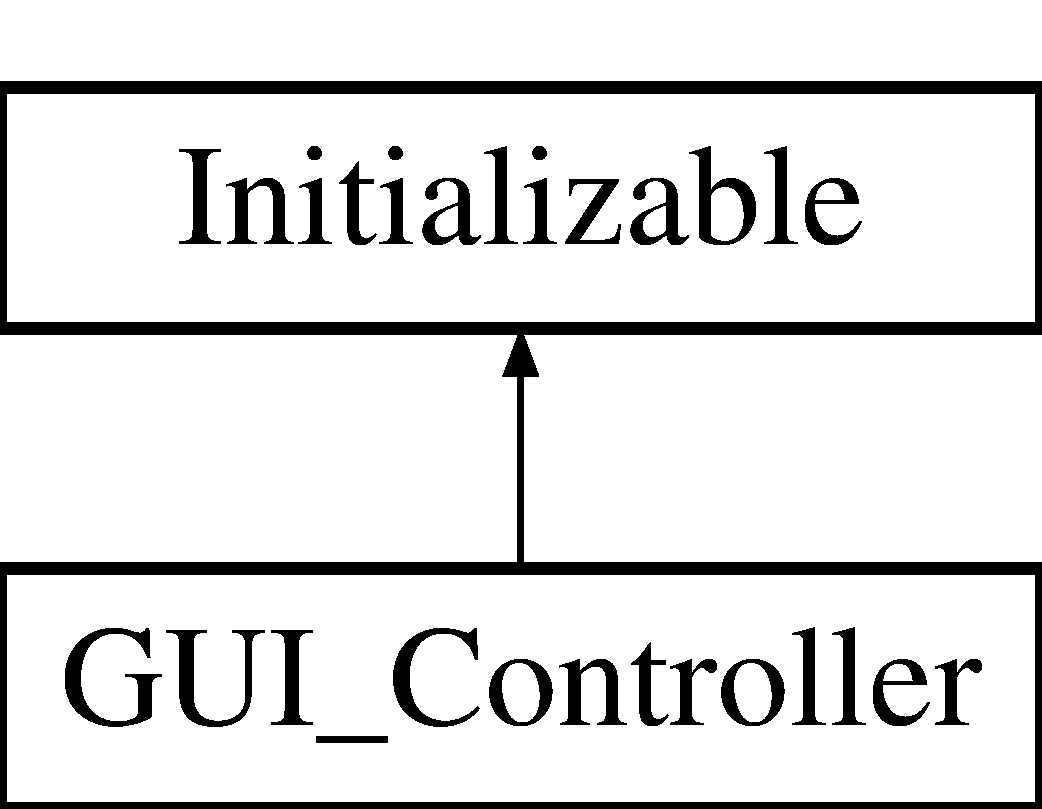
\includegraphics[height=2.000000cm]{classGUI__Controller}
\end{center}
\end{figure}
\subsubsection*{Public Member Functions}
\begin{DoxyCompactItemize}
\item 
\mbox{\Hypertarget{classGUI__Controller_aca7a1ba9eac5b2cd4e2aba8e84c478d8}\label{classGUI__Controller_aca7a1ba9eac5b2cd4e2aba8e84c478d8}} 
void {\bfseries initialize} (U\+RL url, Resource\+Bundle rb)
\end{DoxyCompactItemize}
\subsubsection*{Private Member Functions}
\begin{DoxyCompactItemize}
\item 
void \hyperlink{classGUI__Controller_a19c63367b86511e65296208c8cacb030}{zero\+Action} (Action\+Event event)
\begin{DoxyCompactList}\small\item\em Zero button pressed. \end{DoxyCompactList}\item 
void \hyperlink{classGUI__Controller_a90e608ef1790b4744312cafbb33d7d9c}{one\+Action} (Action\+Event event)
\begin{DoxyCompactList}\small\item\em Button \textquotesingle{}1\textquotesingle{} pressed. \end{DoxyCompactList}\item 
void \hyperlink{classGUI__Controller_a71317bb436ee46213733eaec13dd6ab8}{two\+Action} (Action\+Event event)
\begin{DoxyCompactList}\small\item\em Button \textquotesingle{}2\textquotesingle{} pressed. \end{DoxyCompactList}\item 
void \hyperlink{classGUI__Controller_a545e88d3e80c4b250eaa8254d18c43e6}{three\+Action} (Action\+Event event)
\begin{DoxyCompactList}\small\item\em Button \textquotesingle{}3\textquotesingle{} pressed. \end{DoxyCompactList}\item 
void \hyperlink{classGUI__Controller_a98a563cfbb9c2a951ee786d576a2329c}{four\+Action} (Action\+Event event)
\begin{DoxyCompactList}\small\item\em Button \textquotesingle{}4\textquotesingle{} pressed. \end{DoxyCompactList}\item 
void \hyperlink{classGUI__Controller_a9066c255f0d91d630948ab792319d59d}{five\+Action} (Action\+Event event)
\begin{DoxyCompactList}\small\item\em Button \textquotesingle{}5\textquotesingle{} pressed. \end{DoxyCompactList}\item 
void \hyperlink{classGUI__Controller_a7d45a1041c32ff8ca5e721c56651fe49}{six\+Action} (Action\+Event event)
\begin{DoxyCompactList}\small\item\em Button \textquotesingle{}6\textquotesingle{} pressed. \end{DoxyCompactList}\item 
void \hyperlink{classGUI__Controller_a4eece09e941a48b35c7c4e067ee02317}{seven\+Action} (Action\+Event event)
\begin{DoxyCompactList}\small\item\em Button \textquotesingle{}7\textquotesingle{} pressed. \end{DoxyCompactList}\item 
void \hyperlink{classGUI__Controller_a8688f22bd92312d2e1b9c1d74df7e7fc}{eigth\+Action} (Action\+Event event)
\begin{DoxyCompactList}\small\item\em Button \textquotesingle{}8\textquotesingle{} pressed. \end{DoxyCompactList}\item 
void \hyperlink{classGUI__Controller_aa5e4b5629d363e264f832c0d17b04d4b}{nine\+Action} (Action\+Event event)
\begin{DoxyCompactList}\small\item\em Button \textquotesingle{}9\textquotesingle{} pressed. \end{DoxyCompactList}\item 
void \hyperlink{classGUI__Controller_a491246305bbe61ee5267a9b3a06fb3cb}{D\+E\+L\+Action} (Action\+Event event)
\begin{DoxyCompactList}\small\item\em Button \textquotesingle{}D\+EL\textquotesingle{} pressed. \end{DoxyCompactList}\item 
void \hyperlink{classGUI__Controller_a33eaf846c2f54a13fcdf8a4e0dfb98d0}{C\+Action} (Action\+Event event)
\begin{DoxyCompactList}\small\item\em Button \textquotesingle{}CA\textquotesingle{} pressed. \end{DoxyCompactList}\item 
void \hyperlink{classGUI__Controller_a5ab4d097a40e0ea15392c65757a052aa}{equal\+Action} (Action\+Event event)
\begin{DoxyCompactList}\small\item\em Button \textquotesingle{}=\textquotesingle{} pressed. \end{DoxyCompactList}\item 
void \hyperlink{classGUI__Controller_abab880a50c742388974a9f96e147e1f5}{dot\+Action} (Action\+Event event)
\begin{DoxyCompactList}\small\item\em Button \textquotesingle{}.\textquotesingle{} pressed. \end{DoxyCompactList}\item 
void \hyperlink{classGUI__Controller_a1a2f902a1462a48bf26769d4ee3689c7}{plus\+Action} (Action\+Event event)
\begin{DoxyCompactList}\small\item\em Button \textquotesingle{}+\textquotesingle{} pressed. \end{DoxyCompactList}\item 
void \hyperlink{classGUI__Controller_a01a8f10c74c34426cd923b699d5da5b3}{minus\+Action} (Action\+Event event)
\begin{DoxyCompactList}\small\item\em Button \textquotesingle{}-\/\textquotesingle{} pressed. \end{DoxyCompactList}\item 
void \hyperlink{classGUI__Controller_a0a15fea5ff39777ca3ec7f52e5d35500}{modulo\+Action} (Action\+Event event)
\begin{DoxyCompactList}\small\item\em Button \textquotesingle{}\textquotesingle{} pressed. \end{DoxyCompactList}\item 
void \hyperlink{classGUI__Controller_a504ebbabf072956cac740e9fdc4e68c9}{sqrt\+Action} (Action\+Event event)
\begin{DoxyCompactList}\small\item\em Button \textquotesingle{}sqrt\textquotesingle{} pressed. \end{DoxyCompactList}\item 
void \hyperlink{classGUI__Controller_a5d06ebc913880c0166c64ce44820ede5}{pow\+Action} (Action\+Event event)
\begin{DoxyCompactList}\small\item\em Button \textquotesingle{}$^\wedge$\textquotesingle{} pressed. \end{DoxyCompactList}\item 
void \hyperlink{classGUI__Controller_a3e8f8e68324279d1a1ca47b25f76bd03}{multi\+Action} (Action\+Event event)
\begin{DoxyCompactList}\small\item\em Button \textquotesingle{}$\ast$\textquotesingle{} pressed. \end{DoxyCompactList}\item 
void \hyperlink{classGUI__Controller_aa8ff04e83edf0943671173ccb7fcb716}{div\+Action} (Action\+Event event)
\begin{DoxyCompactList}\small\item\em Button \textquotesingle{}/\textquotesingle{} pressed. \end{DoxyCompactList}\item 
void \hyperlink{classGUI__Controller_a254bda9a37fb413e27572c045b6329f6}{fact\+Action} (Action\+Event event)
\begin{DoxyCompactList}\small\item\em Button \textquotesingle{}!\textquotesingle{} pressed. \end{DoxyCompactList}\item 
void \hyperlink{classGUI__Controller_aeaa83c7bf60a12582636385571d1241a}{help\+Action} (Action\+Event event)
\begin{DoxyCompactList}\small\item\em Button \textquotesingle{}?\textquotesingle{} pressed. \end{DoxyCompactList}\item 
\mbox{\Hypertarget{classGUI__Controller_a152911421c341bb77bfa6e4e1d227d79}\label{classGUI__Controller_a152911421c341bb77bfa6e4e1d227d79}} 
void \hyperlink{classGUI__Controller_a152911421c341bb77bfa6e4e1d227d79}{mid\+\_\+result} ()
\begin{DoxyCompactList}\small\item\em Function handling more than one operation in row. \end{DoxyCompactList}\item 
long \hyperlink{classGUI__Controller_aff1ce595ea2abf5309f8225126e912db}{is\+\_\+int} (double x)
\begin{DoxyCompactList}\small\item\em Function will chceck whether the given number is integer or not. \end{DoxyCompactList}\item 
\mbox{\Hypertarget{classGUI__Controller_ac879b351de7c6f032825558ee179237e}\label{classGUI__Controller_ac879b351de7c6f032825558ee179237e}} 
void \hyperlink{classGUI__Controller_ac879b351de7c6f032825558ee179237e}{reset} ()
\begin{DoxyCompactList}\small\item\em noooo idea \end{DoxyCompactList}\end{DoxyCompactItemize}
\subsubsection*{Private Attributes}
\begin{DoxyCompactItemize}
\item 
\mbox{\Hypertarget{classGUI__Controller_aa756d9f66302e6328e78d72edd55ac18}\label{classGUI__Controller_aa756d9f66302e6328e78d72edd55ac18}} 
Text\+Field {\bfseries display}
\item 
\mbox{\Hypertarget{classGUI__Controller_aa021522bb2112a326ae8461a677130c4}\label{classGUI__Controller_aa021522bb2112a326ae8461a677130c4}} 
Text\+Field {\bfseries O\+P\+\_\+display}
\item 
\mbox{\Hypertarget{classGUI__Controller_a2bcbaa0c0c3b82ee2a45869bfe14562b}\label{classGUI__Controller_a2bcbaa0c0c3b82ee2a45869bfe14562b}} 
double {\bfseries operand\+\_\+one}
\item 
\mbox{\Hypertarget{classGUI__Controller_a0aefa5e433461b7d0e2649a58f2ca2d9}\label{classGUI__Controller_a0aefa5e433461b7d0e2649a58f2ca2d9}} 
double {\bfseries operand\+\_\+two}
\item 
\mbox{\Hypertarget{classGUI__Controller_af0ace5297c907a30a11cef1dea65a908}\label{classGUI__Controller_af0ace5297c907a30a11cef1dea65a908}} 
boolean {\bfseries dot\+\_\+flag}
\item 
\mbox{\Hypertarget{classGUI__Controller_ae270f6e868d0fd41b1bd3aae0ad8971f}\label{classGUI__Controller_ae270f6e868d0fd41b1bd3aae0ad8971f}} 
boolean {\bfseries reset\+\_\+D}
\item 
\mbox{\Hypertarget{classGUI__Controller_a981626a034c144c31db9ed51a1e203a3}\label{classGUI__Controller_a981626a034c144c31db9ed51a1e203a3}} 
int {\bfseries operation}
\end{DoxyCompactItemize}


\subsubsection{Member Function Documentation}
\mbox{\Hypertarget{classGUI__Controller_a33eaf846c2f54a13fcdf8a4e0dfb98d0}\label{classGUI__Controller_a33eaf846c2f54a13fcdf8a4e0dfb98d0}} 
\index{G\+U\+I\+\_\+\+Controller@{G\+U\+I\+\_\+\+Controller}!C\+Action@{C\+Action}}
\index{C\+Action@{C\+Action}!G\+U\+I\+\_\+\+Controller@{G\+U\+I\+\_\+\+Controller}}
\paragraph{\texorpdfstring{C\+Action()}{CAction()}}
{\footnotesize\ttfamily void G\+U\+I\+\_\+\+Controller.\+C\+Action (\begin{DoxyParamCaption}\item[{Action\+Event}]{event }\end{DoxyParamCaption})\hspace{0.3cm}{\ttfamily [inline]}, {\ttfamily [private]}}



Button \textquotesingle{}CA\textquotesingle{} pressed. 


\begin{DoxyParams}{Parameters}
{\em event} & todo \\
\hline
\end{DoxyParams}
\mbox{\Hypertarget{classGUI__Controller_a491246305bbe61ee5267a9b3a06fb3cb}\label{classGUI__Controller_a491246305bbe61ee5267a9b3a06fb3cb}} 
\index{G\+U\+I\+\_\+\+Controller@{G\+U\+I\+\_\+\+Controller}!D\+E\+L\+Action@{D\+E\+L\+Action}}
\index{D\+E\+L\+Action@{D\+E\+L\+Action}!G\+U\+I\+\_\+\+Controller@{G\+U\+I\+\_\+\+Controller}}
\paragraph{\texorpdfstring{D\+E\+L\+Action()}{DELAction()}}
{\footnotesize\ttfamily void G\+U\+I\+\_\+\+Controller.\+D\+E\+L\+Action (\begin{DoxyParamCaption}\item[{Action\+Event}]{event }\end{DoxyParamCaption})\hspace{0.3cm}{\ttfamily [inline]}, {\ttfamily [private]}}



Button \textquotesingle{}D\+EL\textquotesingle{} pressed. 


\begin{DoxyParams}{Parameters}
{\em event} & todo \\
\hline
\end{DoxyParams}
\mbox{\Hypertarget{classGUI__Controller_aa8ff04e83edf0943671173ccb7fcb716}\label{classGUI__Controller_aa8ff04e83edf0943671173ccb7fcb716}} 
\index{G\+U\+I\+\_\+\+Controller@{G\+U\+I\+\_\+\+Controller}!div\+Action@{div\+Action}}
\index{div\+Action@{div\+Action}!G\+U\+I\+\_\+\+Controller@{G\+U\+I\+\_\+\+Controller}}
\paragraph{\texorpdfstring{div\+Action()}{divAction()}}
{\footnotesize\ttfamily void G\+U\+I\+\_\+\+Controller.\+div\+Action (\begin{DoxyParamCaption}\item[{Action\+Event}]{event }\end{DoxyParamCaption})\hspace{0.3cm}{\ttfamily [inline]}, {\ttfamily [private]}}



Button \textquotesingle{}/\textquotesingle{} pressed. 


\begin{DoxyParams}{Parameters}
{\em event} & todo \\
\hline
\end{DoxyParams}
\mbox{\Hypertarget{classGUI__Controller_abab880a50c742388974a9f96e147e1f5}\label{classGUI__Controller_abab880a50c742388974a9f96e147e1f5}} 
\index{G\+U\+I\+\_\+\+Controller@{G\+U\+I\+\_\+\+Controller}!dot\+Action@{dot\+Action}}
\index{dot\+Action@{dot\+Action}!G\+U\+I\+\_\+\+Controller@{G\+U\+I\+\_\+\+Controller}}
\paragraph{\texorpdfstring{dot\+Action()}{dotAction()}}
{\footnotesize\ttfamily void G\+U\+I\+\_\+\+Controller.\+dot\+Action (\begin{DoxyParamCaption}\item[{Action\+Event}]{event }\end{DoxyParamCaption})\hspace{0.3cm}{\ttfamily [inline]}, {\ttfamily [private]}}



Button \textquotesingle{}.\textquotesingle{} pressed. 


\begin{DoxyParams}{Parameters}
{\em event} & todo \\
\hline
\end{DoxyParams}
\mbox{\Hypertarget{classGUI__Controller_a8688f22bd92312d2e1b9c1d74df7e7fc}\label{classGUI__Controller_a8688f22bd92312d2e1b9c1d74df7e7fc}} 
\index{G\+U\+I\+\_\+\+Controller@{G\+U\+I\+\_\+\+Controller}!eigth\+Action@{eigth\+Action}}
\index{eigth\+Action@{eigth\+Action}!G\+U\+I\+\_\+\+Controller@{G\+U\+I\+\_\+\+Controller}}
\paragraph{\texorpdfstring{eigth\+Action()}{eigthAction()}}
{\footnotesize\ttfamily void G\+U\+I\+\_\+\+Controller.\+eigth\+Action (\begin{DoxyParamCaption}\item[{Action\+Event}]{event }\end{DoxyParamCaption})\hspace{0.3cm}{\ttfamily [inline]}, {\ttfamily [private]}}



Button \textquotesingle{}8\textquotesingle{} pressed. 


\begin{DoxyParams}{Parameters}
{\em event} & todo \\
\hline
\end{DoxyParams}
\mbox{\Hypertarget{classGUI__Controller_a5ab4d097a40e0ea15392c65757a052aa}\label{classGUI__Controller_a5ab4d097a40e0ea15392c65757a052aa}} 
\index{G\+U\+I\+\_\+\+Controller@{G\+U\+I\+\_\+\+Controller}!equal\+Action@{equal\+Action}}
\index{equal\+Action@{equal\+Action}!G\+U\+I\+\_\+\+Controller@{G\+U\+I\+\_\+\+Controller}}
\paragraph{\texorpdfstring{equal\+Action()}{equalAction()}}
{\footnotesize\ttfamily void G\+U\+I\+\_\+\+Controller.\+equal\+Action (\begin{DoxyParamCaption}\item[{Action\+Event}]{event }\end{DoxyParamCaption})\hspace{0.3cm}{\ttfamily [inline]}, {\ttfamily [private]}}



Button \textquotesingle{}=\textquotesingle{} pressed. 


\begin{DoxyParams}{Parameters}
{\em event} & todo \\
\hline
\end{DoxyParams}
\mbox{\Hypertarget{classGUI__Controller_a254bda9a37fb413e27572c045b6329f6}\label{classGUI__Controller_a254bda9a37fb413e27572c045b6329f6}} 
\index{G\+U\+I\+\_\+\+Controller@{G\+U\+I\+\_\+\+Controller}!fact\+Action@{fact\+Action}}
\index{fact\+Action@{fact\+Action}!G\+U\+I\+\_\+\+Controller@{G\+U\+I\+\_\+\+Controller}}
\paragraph{\texorpdfstring{fact\+Action()}{factAction()}}
{\footnotesize\ttfamily void G\+U\+I\+\_\+\+Controller.\+fact\+Action (\begin{DoxyParamCaption}\item[{Action\+Event}]{event }\end{DoxyParamCaption})\hspace{0.3cm}{\ttfamily [inline]}, {\ttfamily [private]}}



Button \textquotesingle{}!\textquotesingle{} pressed. 


\begin{DoxyParams}{Parameters}
{\em event} & todo \\
\hline
\end{DoxyParams}
\mbox{\Hypertarget{classGUI__Controller_a9066c255f0d91d630948ab792319d59d}\label{classGUI__Controller_a9066c255f0d91d630948ab792319d59d}} 
\index{G\+U\+I\+\_\+\+Controller@{G\+U\+I\+\_\+\+Controller}!five\+Action@{five\+Action}}
\index{five\+Action@{five\+Action}!G\+U\+I\+\_\+\+Controller@{G\+U\+I\+\_\+\+Controller}}
\paragraph{\texorpdfstring{five\+Action()}{fiveAction()}}
{\footnotesize\ttfamily void G\+U\+I\+\_\+\+Controller.\+five\+Action (\begin{DoxyParamCaption}\item[{Action\+Event}]{event }\end{DoxyParamCaption})\hspace{0.3cm}{\ttfamily [inline]}, {\ttfamily [private]}}



Button \textquotesingle{}5\textquotesingle{} pressed. 


\begin{DoxyParams}{Parameters}
{\em event} & todo \\
\hline
\end{DoxyParams}
\mbox{\Hypertarget{classGUI__Controller_a98a563cfbb9c2a951ee786d576a2329c}\label{classGUI__Controller_a98a563cfbb9c2a951ee786d576a2329c}} 
\index{G\+U\+I\+\_\+\+Controller@{G\+U\+I\+\_\+\+Controller}!four\+Action@{four\+Action}}
\index{four\+Action@{four\+Action}!G\+U\+I\+\_\+\+Controller@{G\+U\+I\+\_\+\+Controller}}
\paragraph{\texorpdfstring{four\+Action()}{fourAction()}}
{\footnotesize\ttfamily void G\+U\+I\+\_\+\+Controller.\+four\+Action (\begin{DoxyParamCaption}\item[{Action\+Event}]{event }\end{DoxyParamCaption})\hspace{0.3cm}{\ttfamily [inline]}, {\ttfamily [private]}}



Button \textquotesingle{}4\textquotesingle{} pressed. 


\begin{DoxyParams}{Parameters}
{\em event} & todo \\
\hline
\end{DoxyParams}
\mbox{\Hypertarget{classGUI__Controller_aeaa83c7bf60a12582636385571d1241a}\label{classGUI__Controller_aeaa83c7bf60a12582636385571d1241a}} 
\index{G\+U\+I\+\_\+\+Controller@{G\+U\+I\+\_\+\+Controller}!help\+Action@{help\+Action}}
\index{help\+Action@{help\+Action}!G\+U\+I\+\_\+\+Controller@{G\+U\+I\+\_\+\+Controller}}
\paragraph{\texorpdfstring{help\+Action()}{helpAction()}}
{\footnotesize\ttfamily void G\+U\+I\+\_\+\+Controller.\+help\+Action (\begin{DoxyParamCaption}\item[{Action\+Event}]{event }\end{DoxyParamCaption})\hspace{0.3cm}{\ttfamily [inline]}, {\ttfamily [private]}}



Button \textquotesingle{}?\textquotesingle{} pressed. 


\begin{DoxyParams}{Parameters}
{\em event} & todo \\
\hline
\end{DoxyParams}
\mbox{\Hypertarget{classGUI__Controller_aff1ce595ea2abf5309f8225126e912db}\label{classGUI__Controller_aff1ce595ea2abf5309f8225126e912db}} 
\index{G\+U\+I\+\_\+\+Controller@{G\+U\+I\+\_\+\+Controller}!is\+\_\+int@{is\+\_\+int}}
\index{is\+\_\+int@{is\+\_\+int}!G\+U\+I\+\_\+\+Controller@{G\+U\+I\+\_\+\+Controller}}
\paragraph{\texorpdfstring{is\+\_\+int()}{is\_int()}}
{\footnotesize\ttfamily long G\+U\+I\+\_\+\+Controller.\+is\+\_\+int (\begin{DoxyParamCaption}\item[{double}]{x }\end{DoxyParamCaption})\hspace{0.3cm}{\ttfamily [inline]}, {\ttfamily [private]}}



Function will chceck whether the given number is integer or not. 


\begin{DoxyParams}{Parameters}
{\em x} & Number to be checked. \\
\hline
\end{DoxyParams}
\begin{DoxyReturn}{Returns}
Integer representation of number if number was x.\+0, or -\/1 if not. 
\end{DoxyReturn}
\mbox{\Hypertarget{classGUI__Controller_a01a8f10c74c34426cd923b699d5da5b3}\label{classGUI__Controller_a01a8f10c74c34426cd923b699d5da5b3}} 
\index{G\+U\+I\+\_\+\+Controller@{G\+U\+I\+\_\+\+Controller}!minus\+Action@{minus\+Action}}
\index{minus\+Action@{minus\+Action}!G\+U\+I\+\_\+\+Controller@{G\+U\+I\+\_\+\+Controller}}
\paragraph{\texorpdfstring{minus\+Action()}{minusAction()}}
{\footnotesize\ttfamily void G\+U\+I\+\_\+\+Controller.\+minus\+Action (\begin{DoxyParamCaption}\item[{Action\+Event}]{event }\end{DoxyParamCaption})\hspace{0.3cm}{\ttfamily [inline]}, {\ttfamily [private]}}



Button \textquotesingle{}-\/\textquotesingle{} pressed. 


\begin{DoxyParams}{Parameters}
{\em event} & todo \\
\hline
\end{DoxyParams}
\mbox{\Hypertarget{classGUI__Controller_a0a15fea5ff39777ca3ec7f52e5d35500}\label{classGUI__Controller_a0a15fea5ff39777ca3ec7f52e5d35500}} 
\index{G\+U\+I\+\_\+\+Controller@{G\+U\+I\+\_\+\+Controller}!modulo\+Action@{modulo\+Action}}
\index{modulo\+Action@{modulo\+Action}!G\+U\+I\+\_\+\+Controller@{G\+U\+I\+\_\+\+Controller}}
\paragraph{\texorpdfstring{modulo\+Action()}{moduloAction()}}
{\footnotesize\ttfamily void G\+U\+I\+\_\+\+Controller.\+modulo\+Action (\begin{DoxyParamCaption}\item[{Action\+Event}]{event }\end{DoxyParamCaption})\hspace{0.3cm}{\ttfamily [inline]}, {\ttfamily [private]}}



Button \textquotesingle{}\textquotesingle{} pressed. 


\begin{DoxyParams}{Parameters}
{\em event} & todo \\
\hline
\end{DoxyParams}
\mbox{\Hypertarget{classGUI__Controller_a3e8f8e68324279d1a1ca47b25f76bd03}\label{classGUI__Controller_a3e8f8e68324279d1a1ca47b25f76bd03}} 
\index{G\+U\+I\+\_\+\+Controller@{G\+U\+I\+\_\+\+Controller}!multi\+Action@{multi\+Action}}
\index{multi\+Action@{multi\+Action}!G\+U\+I\+\_\+\+Controller@{G\+U\+I\+\_\+\+Controller}}
\paragraph{\texorpdfstring{multi\+Action()}{multiAction()}}
{\footnotesize\ttfamily void G\+U\+I\+\_\+\+Controller.\+multi\+Action (\begin{DoxyParamCaption}\item[{Action\+Event}]{event }\end{DoxyParamCaption})\hspace{0.3cm}{\ttfamily [inline]}, {\ttfamily [private]}}



Button \textquotesingle{}$\ast$\textquotesingle{} pressed. 


\begin{DoxyParams}{Parameters}
{\em event} & todo \\
\hline
\end{DoxyParams}
\mbox{\Hypertarget{classGUI__Controller_aa5e4b5629d363e264f832c0d17b04d4b}\label{classGUI__Controller_aa5e4b5629d363e264f832c0d17b04d4b}} 
\index{G\+U\+I\+\_\+\+Controller@{G\+U\+I\+\_\+\+Controller}!nine\+Action@{nine\+Action}}
\index{nine\+Action@{nine\+Action}!G\+U\+I\+\_\+\+Controller@{G\+U\+I\+\_\+\+Controller}}
\paragraph{\texorpdfstring{nine\+Action()}{nineAction()}}
{\footnotesize\ttfamily void G\+U\+I\+\_\+\+Controller.\+nine\+Action (\begin{DoxyParamCaption}\item[{Action\+Event}]{event }\end{DoxyParamCaption})\hspace{0.3cm}{\ttfamily [inline]}, {\ttfamily [private]}}



Button \textquotesingle{}9\textquotesingle{} pressed. 


\begin{DoxyParams}{Parameters}
{\em event} & todo \\
\hline
\end{DoxyParams}
\mbox{\Hypertarget{classGUI__Controller_a90e608ef1790b4744312cafbb33d7d9c}\label{classGUI__Controller_a90e608ef1790b4744312cafbb33d7d9c}} 
\index{G\+U\+I\+\_\+\+Controller@{G\+U\+I\+\_\+\+Controller}!one\+Action@{one\+Action}}
\index{one\+Action@{one\+Action}!G\+U\+I\+\_\+\+Controller@{G\+U\+I\+\_\+\+Controller}}
\paragraph{\texorpdfstring{one\+Action()}{oneAction()}}
{\footnotesize\ttfamily void G\+U\+I\+\_\+\+Controller.\+one\+Action (\begin{DoxyParamCaption}\item[{Action\+Event}]{event }\end{DoxyParamCaption})\hspace{0.3cm}{\ttfamily [inline]}, {\ttfamily [private]}}



Button \textquotesingle{}1\textquotesingle{} pressed. 


\begin{DoxyParams}{Parameters}
{\em event} & todo \\
\hline
\end{DoxyParams}
\mbox{\Hypertarget{classGUI__Controller_a1a2f902a1462a48bf26769d4ee3689c7}\label{classGUI__Controller_a1a2f902a1462a48bf26769d4ee3689c7}} 
\index{G\+U\+I\+\_\+\+Controller@{G\+U\+I\+\_\+\+Controller}!plus\+Action@{plus\+Action}}
\index{plus\+Action@{plus\+Action}!G\+U\+I\+\_\+\+Controller@{G\+U\+I\+\_\+\+Controller}}
\paragraph{\texorpdfstring{plus\+Action()}{plusAction()}}
{\footnotesize\ttfamily void G\+U\+I\+\_\+\+Controller.\+plus\+Action (\begin{DoxyParamCaption}\item[{Action\+Event}]{event }\end{DoxyParamCaption})\hspace{0.3cm}{\ttfamily [inline]}, {\ttfamily [private]}}



Button \textquotesingle{}+\textquotesingle{} pressed. 


\begin{DoxyParams}{Parameters}
{\em event} & todo \\
\hline
\end{DoxyParams}
\mbox{\Hypertarget{classGUI__Controller_a5d06ebc913880c0166c64ce44820ede5}\label{classGUI__Controller_a5d06ebc913880c0166c64ce44820ede5}} 
\index{G\+U\+I\+\_\+\+Controller@{G\+U\+I\+\_\+\+Controller}!pow\+Action@{pow\+Action}}
\index{pow\+Action@{pow\+Action}!G\+U\+I\+\_\+\+Controller@{G\+U\+I\+\_\+\+Controller}}
\paragraph{\texorpdfstring{pow\+Action()}{powAction()}}
{\footnotesize\ttfamily void G\+U\+I\+\_\+\+Controller.\+pow\+Action (\begin{DoxyParamCaption}\item[{Action\+Event}]{event }\end{DoxyParamCaption})\hspace{0.3cm}{\ttfamily [inline]}, {\ttfamily [private]}}



Button \textquotesingle{}$^\wedge$\textquotesingle{} pressed. 


\begin{DoxyParams}{Parameters}
{\em event} & todo \\
\hline
\end{DoxyParams}
\mbox{\Hypertarget{classGUI__Controller_a4eece09e941a48b35c7c4e067ee02317}\label{classGUI__Controller_a4eece09e941a48b35c7c4e067ee02317}} 
\index{G\+U\+I\+\_\+\+Controller@{G\+U\+I\+\_\+\+Controller}!seven\+Action@{seven\+Action}}
\index{seven\+Action@{seven\+Action}!G\+U\+I\+\_\+\+Controller@{G\+U\+I\+\_\+\+Controller}}
\paragraph{\texorpdfstring{seven\+Action()}{sevenAction()}}
{\footnotesize\ttfamily void G\+U\+I\+\_\+\+Controller.\+seven\+Action (\begin{DoxyParamCaption}\item[{Action\+Event}]{event }\end{DoxyParamCaption})\hspace{0.3cm}{\ttfamily [inline]}, {\ttfamily [private]}}



Button \textquotesingle{}7\textquotesingle{} pressed. 


\begin{DoxyParams}{Parameters}
{\em event} & todo \\
\hline
\end{DoxyParams}
\mbox{\Hypertarget{classGUI__Controller_a7d45a1041c32ff8ca5e721c56651fe49}\label{classGUI__Controller_a7d45a1041c32ff8ca5e721c56651fe49}} 
\index{G\+U\+I\+\_\+\+Controller@{G\+U\+I\+\_\+\+Controller}!six\+Action@{six\+Action}}
\index{six\+Action@{six\+Action}!G\+U\+I\+\_\+\+Controller@{G\+U\+I\+\_\+\+Controller}}
\paragraph{\texorpdfstring{six\+Action()}{sixAction()}}
{\footnotesize\ttfamily void G\+U\+I\+\_\+\+Controller.\+six\+Action (\begin{DoxyParamCaption}\item[{Action\+Event}]{event }\end{DoxyParamCaption})\hspace{0.3cm}{\ttfamily [inline]}, {\ttfamily [private]}}



Button \textquotesingle{}6\textquotesingle{} pressed. 


\begin{DoxyParams}{Parameters}
{\em event} & todo \\
\hline
\end{DoxyParams}
\mbox{\Hypertarget{classGUI__Controller_a504ebbabf072956cac740e9fdc4e68c9}\label{classGUI__Controller_a504ebbabf072956cac740e9fdc4e68c9}} 
\index{G\+U\+I\+\_\+\+Controller@{G\+U\+I\+\_\+\+Controller}!sqrt\+Action@{sqrt\+Action}}
\index{sqrt\+Action@{sqrt\+Action}!G\+U\+I\+\_\+\+Controller@{G\+U\+I\+\_\+\+Controller}}
\paragraph{\texorpdfstring{sqrt\+Action()}{sqrtAction()}}
{\footnotesize\ttfamily void G\+U\+I\+\_\+\+Controller.\+sqrt\+Action (\begin{DoxyParamCaption}\item[{Action\+Event}]{event }\end{DoxyParamCaption})\hspace{0.3cm}{\ttfamily [inline]}, {\ttfamily [private]}}



Button \textquotesingle{}sqrt\textquotesingle{} pressed. 


\begin{DoxyParams}{Parameters}
{\em event} & todo \\
\hline
\end{DoxyParams}
\mbox{\Hypertarget{classGUI__Controller_a545e88d3e80c4b250eaa8254d18c43e6}\label{classGUI__Controller_a545e88d3e80c4b250eaa8254d18c43e6}} 
\index{G\+U\+I\+\_\+\+Controller@{G\+U\+I\+\_\+\+Controller}!three\+Action@{three\+Action}}
\index{three\+Action@{three\+Action}!G\+U\+I\+\_\+\+Controller@{G\+U\+I\+\_\+\+Controller}}
\paragraph{\texorpdfstring{three\+Action()}{threeAction()}}
{\footnotesize\ttfamily void G\+U\+I\+\_\+\+Controller.\+three\+Action (\begin{DoxyParamCaption}\item[{Action\+Event}]{event }\end{DoxyParamCaption})\hspace{0.3cm}{\ttfamily [inline]}, {\ttfamily [private]}}



Button \textquotesingle{}3\textquotesingle{} pressed. 


\begin{DoxyParams}{Parameters}
{\em event} & todo \\
\hline
\end{DoxyParams}
\mbox{\Hypertarget{classGUI__Controller_a71317bb436ee46213733eaec13dd6ab8}\label{classGUI__Controller_a71317bb436ee46213733eaec13dd6ab8}} 
\index{G\+U\+I\+\_\+\+Controller@{G\+U\+I\+\_\+\+Controller}!two\+Action@{two\+Action}}
\index{two\+Action@{two\+Action}!G\+U\+I\+\_\+\+Controller@{G\+U\+I\+\_\+\+Controller}}
\paragraph{\texorpdfstring{two\+Action()}{twoAction()}}
{\footnotesize\ttfamily void G\+U\+I\+\_\+\+Controller.\+two\+Action (\begin{DoxyParamCaption}\item[{Action\+Event}]{event }\end{DoxyParamCaption})\hspace{0.3cm}{\ttfamily [inline]}, {\ttfamily [private]}}



Button \textquotesingle{}2\textquotesingle{} pressed. 


\begin{DoxyParams}{Parameters}
{\em event} & todo \\
\hline
\end{DoxyParams}
\mbox{\Hypertarget{classGUI__Controller_a19c63367b86511e65296208c8cacb030}\label{classGUI__Controller_a19c63367b86511e65296208c8cacb030}} 
\index{G\+U\+I\+\_\+\+Controller@{G\+U\+I\+\_\+\+Controller}!zero\+Action@{zero\+Action}}
\index{zero\+Action@{zero\+Action}!G\+U\+I\+\_\+\+Controller@{G\+U\+I\+\_\+\+Controller}}
\paragraph{\texorpdfstring{zero\+Action()}{zeroAction()}}
{\footnotesize\ttfamily void G\+U\+I\+\_\+\+Controller.\+zero\+Action (\begin{DoxyParamCaption}\item[{Action\+Event}]{event }\end{DoxyParamCaption})\hspace{0.3cm}{\ttfamily [inline]}, {\ttfamily [private]}}



Zero button pressed. 


\begin{DoxyParams}{Parameters}
{\em event} & todo \\
\hline
\end{DoxyParams}


The documentation for this class was generated from the following file\+:\begin{DoxyCompactItemize}
\item 
src/\hyperlink{GUI__Controller_8java}{G\+U\+I\+\_\+\+Controller.\+java}\end{DoxyCompactItemize}

\hypertarget{classHelp__controller}{}\subsection{Help\+\_\+controller Class Reference}
\label{classHelp__controller}\index{Help\+\_\+controller@{Help\+\_\+controller}}
Inheritance diagram for Help\+\_\+controller\+:\begin{figure}[H]
\begin{center}
\leavevmode
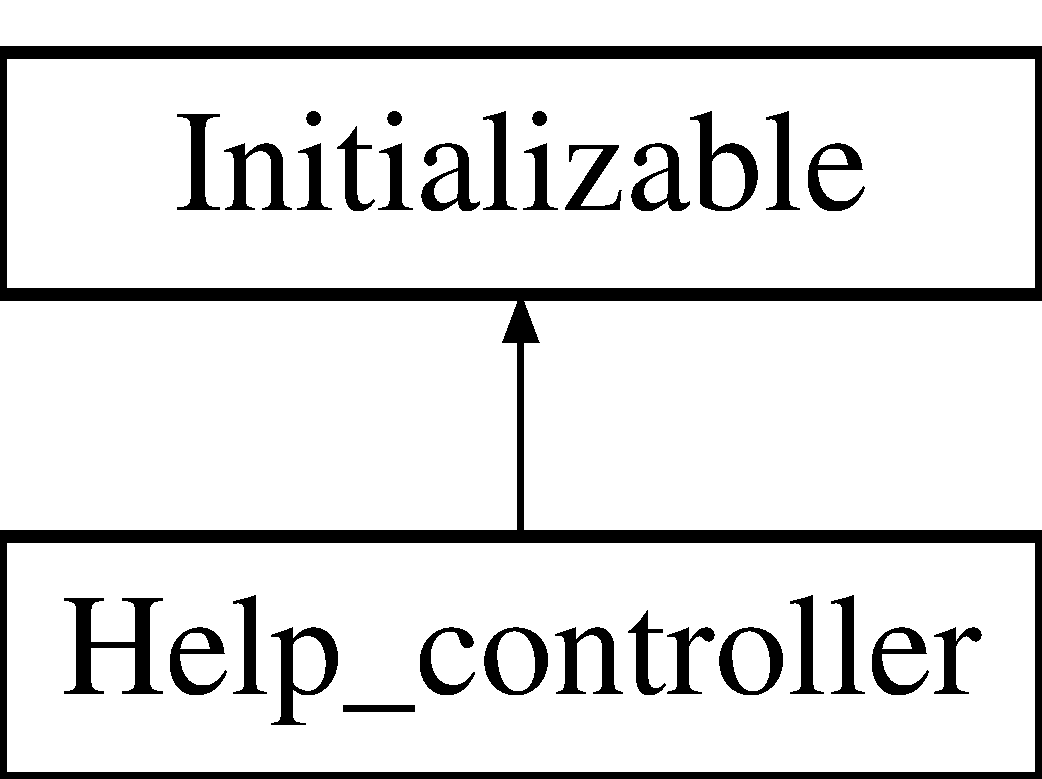
\includegraphics[height=2.000000cm]{classHelp__controller}
\end{center}
\end{figure}
\subsubsection*{Public Member Functions}
\begin{DoxyCompactItemize}
\item 
\mbox{\Hypertarget{classHelp__controller_a645340b84cb76b549a8521ca5a632833}\label{classHelp__controller_a645340b84cb76b549a8521ca5a632833}} 
void {\bfseries initialize} (U\+RL url, Resource\+Bundle rb)
\end{DoxyCompactItemize}
\subsubsection*{Private Member Functions}
\begin{DoxyCompactItemize}
\item 
\mbox{\Hypertarget{classHelp__controller_a292abe6cca2abf78d114402c61db1df6}\label{classHelp__controller_a292abe6cca2abf78d114402c61db1df6}} 
void {\bfseries close\+Action} (Action\+Event event)
\item 
\mbox{\Hypertarget{classHelp__controller_a5636bfb408ced0efc154cd3933f66577}\label{classHelp__controller_a5636bfb408ced0efc154cd3933f66577}} 
void {\bfseries credits\+Action} (Action\+Event event)
\end{DoxyCompactItemize}
\subsubsection*{Private Attributes}
\begin{DoxyCompactItemize}
\item 
\mbox{\Hypertarget{classHelp__controller_aece6ecdcffe2b2b21c7e8a3494de569d}\label{classHelp__controller_aece6ecdcffe2b2b21c7e8a3494de569d}} 
Button {\bfseries close\+Window}
\end{DoxyCompactItemize}


The documentation for this class was generated from the following file\+:\begin{DoxyCompactItemize}
\item 
src/Help\+\_\+controller.\+java\end{DoxyCompactItemize}

\hypertarget{classmath}{}\subsection{math Class Reference}
\label{classmath}\index{math@{math}}
\subsubsection*{Static Public Member Functions}
\begin{DoxyCompactItemize}
\item 
static double \hyperlink{classmath_aedbba5022af9004b0203aea54267aa47}{add} (double x, double y)
\begin{DoxyCompactList}\small\item\em Function will add two double numbers. \end{DoxyCompactList}\item 
static long \hyperlink{classmath_a13ad6680f54a9900e657909c9bd4452e}{add} (long x, long y)
\begin{DoxyCompactList}\small\item\em Function will add two integer numbers. \end{DoxyCompactList}\item 
static double \hyperlink{classmath_a72d851503e310afe7d44b6c24e40aa7a}{add} (double x, long y)
\begin{DoxyCompactList}\small\item\em Function will add two numbers -\/ one integer and one double. \end{DoxyCompactList}\item 
static double \hyperlink{classmath_a2470ffa51c860423010e4550ee7caa4a}{add} (long x, double y)
\begin{DoxyCompactList}\small\item\em Function will add two numbers -\/ one integer and one double. \end{DoxyCompactList}\item 
static double \hyperlink{classmath_a6a9bec211856c5b6cccf6062826ff758}{sub} (double x, double y)
\begin{DoxyCompactList}\small\item\em Substraction of two numbers. \end{DoxyCompactList}\item 
static double \hyperlink{classmath_a2be9a72bde751de9d7b949d2b917d2b0}{multiply} (double x, double y)
\begin{DoxyCompactList}\small\item\em Function will multiply two double numbers. \end{DoxyCompactList}\item 
static long \hyperlink{classmath_a35d65c04f2cc9e4565d4f11294e1d191}{multiply} (long x, long y)
\begin{DoxyCompactList}\small\item\em Function will multiply two integer numbers. \end{DoxyCompactList}\item 
static double \hyperlink{classmath_aedc67ea56f41744708cd85d151cf8973}{multiply} (long x, double y)
\begin{DoxyCompactList}\small\item\em Function will multiply two numbers -\/ one double and one integer. \end{DoxyCompactList}\item 
static double \hyperlink{classmath_afdcf0aa39976744ed21b47697dea0e55}{multiply} (double x, long y)
\begin{DoxyCompactList}\small\item\em Function will multiply two numbers -\/ one double and one integer. \end{DoxyCompactList}\item 
static double \hyperlink{classmath_a52284400f6e457532e27c40b553e4f01}{divide} (double x, double y)
\begin{DoxyCompactList}\small\item\em Division of two numbers. \end{DoxyCompactList}\item 
static long \hyperlink{classmath_acd82ca2b91e16ffd3c74e361d659f890}{factorial} (long num)
\begin{DoxyCompactList}\small\item\em Function will calculate a factorial of a given number. \end{DoxyCompactList}\item 
static double \hyperlink{classmath_ab3dbc5879cf9cb642f8394cea68785c8}{pow} (double x, int y)
\item 
static int \hyperlink{classmath_a4d0742d73c59ffd903e3dcb50744c328}{pow} (int x, int y)
\item 
static long \hyperlink{classmath_a66b6b2c231324eec1c7ccc3919e34768}{mod} (long x, long y)
\begin{DoxyCompactList}\small\item\em Modulo function. \end{DoxyCompactList}\item 
static double \hyperlink{classmath_a9bce1ed75fbc2f3d7051c2a47088754b}{root} (double x, double root)
\begin{DoxyCompactList}\small\item\em Sqrt function. \end{DoxyCompactList}\end{DoxyCompactItemize}


\subsubsection{Member Function Documentation}
\mbox{\Hypertarget{classmath_aedbba5022af9004b0203aea54267aa47}\label{classmath_aedbba5022af9004b0203aea54267aa47}} 
\index{math@{math}!add@{add}}
\index{add@{add}!math@{math}}
\paragraph{\texorpdfstring{add()}{add()}\hspace{0.1cm}{\footnotesize\ttfamily [1/4]}}
{\footnotesize\ttfamily static double math.\+add (\begin{DoxyParamCaption}\item[{double}]{x,  }\item[{double}]{y }\end{DoxyParamCaption})\hspace{0.3cm}{\ttfamily [inline]}, {\ttfamily [static]}}



Function will add two double numbers. 


\begin{DoxyParams}{Parameters}
{\em x} & first number for operation \\
\hline
{\em y} & second number for operation \\
\hline
\end{DoxyParams}
\begin{DoxyReturn}{Returns}
result of adding two parameters 
\end{DoxyReturn}
\mbox{\Hypertarget{classmath_a13ad6680f54a9900e657909c9bd4452e}\label{classmath_a13ad6680f54a9900e657909c9bd4452e}} 
\index{math@{math}!add@{add}}
\index{add@{add}!math@{math}}
\paragraph{\texorpdfstring{add()}{add()}\hspace{0.1cm}{\footnotesize\ttfamily [2/4]}}
{\footnotesize\ttfamily static long math.\+add (\begin{DoxyParamCaption}\item[{long}]{x,  }\item[{long}]{y }\end{DoxyParamCaption})\hspace{0.3cm}{\ttfamily [inline]}, {\ttfamily [static]}}



Function will add two integer numbers. 


\begin{DoxyParams}{Parameters}
{\em x} & first number for operation \\
\hline
{\em y} & second number for operation \\
\hline
\end{DoxyParams}
\begin{DoxyReturn}{Returns}
result of adding two parameters 
\end{DoxyReturn}
\mbox{\Hypertarget{classmath_a72d851503e310afe7d44b6c24e40aa7a}\label{classmath_a72d851503e310afe7d44b6c24e40aa7a}} 
\index{math@{math}!add@{add}}
\index{add@{add}!math@{math}}
\paragraph{\texorpdfstring{add()}{add()}\hspace{0.1cm}{\footnotesize\ttfamily [3/4]}}
{\footnotesize\ttfamily static double math.\+add (\begin{DoxyParamCaption}\item[{double}]{x,  }\item[{long}]{y }\end{DoxyParamCaption})\hspace{0.3cm}{\ttfamily [inline]}, {\ttfamily [static]}}



Function will add two numbers -\/ one integer and one double. 


\begin{DoxyParams}{Parameters}
{\em x} & first number for operation \\
\hline
{\em y} & second number for operation \\
\hline
\end{DoxyParams}
\begin{DoxyReturn}{Returns}
result of adding two parameters 
\end{DoxyReturn}
\mbox{\Hypertarget{classmath_a2470ffa51c860423010e4550ee7caa4a}\label{classmath_a2470ffa51c860423010e4550ee7caa4a}} 
\index{math@{math}!add@{add}}
\index{add@{add}!math@{math}}
\paragraph{\texorpdfstring{add()}{add()}\hspace{0.1cm}{\footnotesize\ttfamily [4/4]}}
{\footnotesize\ttfamily static double math.\+add (\begin{DoxyParamCaption}\item[{long}]{x,  }\item[{double}]{y }\end{DoxyParamCaption})\hspace{0.3cm}{\ttfamily [inline]}, {\ttfamily [static]}}



Function will add two numbers -\/ one integer and one double. 


\begin{DoxyParams}{Parameters}
{\em x} & first number for operation \\
\hline
{\em y} & second number for operation \\
\hline
\end{DoxyParams}
\begin{DoxyReturn}{Returns}
result of adding two parameters 
\end{DoxyReturn}
\mbox{\Hypertarget{classmath_a52284400f6e457532e27c40b553e4f01}\label{classmath_a52284400f6e457532e27c40b553e4f01}} 
\index{math@{math}!divide@{divide}}
\index{divide@{divide}!math@{math}}
\paragraph{\texorpdfstring{divide()}{divide()}}
{\footnotesize\ttfamily static double math.\+divide (\begin{DoxyParamCaption}\item[{double}]{x,  }\item[{double}]{y }\end{DoxyParamCaption})\hspace{0.3cm}{\ttfamily [inline]}, {\ttfamily [static]}}



Division of two numbers. 


\begin{DoxyParams}{Parameters}
{\em x} & divident \\
\hline
{\em y} & divisor \\
\hline
\end{DoxyParams}
\begin{DoxyReturn}{Returns}
result of dividing two numbers 
\end{DoxyReturn}
\mbox{\Hypertarget{classmath_acd82ca2b91e16ffd3c74e361d659f890}\label{classmath_acd82ca2b91e16ffd3c74e361d659f890}} 
\index{math@{math}!factorial@{factorial}}
\index{factorial@{factorial}!math@{math}}
\paragraph{\texorpdfstring{factorial()}{factorial()}}
{\footnotesize\ttfamily static long math.\+factorial (\begin{DoxyParamCaption}\item[{long}]{num }\end{DoxyParamCaption})\hspace{0.3cm}{\ttfamily [inline]}, {\ttfamily [static]}}



Function will calculate a factorial of a given number. 


\begin{DoxyParams}{Parameters}
{\em num} & number from which we want factorial to be calculated from \\
\hline
\end{DoxyParams}
\begin{DoxyReturn}{Returns}
value of the factorial 
\end{DoxyReturn}
\mbox{\Hypertarget{classmath_a66b6b2c231324eec1c7ccc3919e34768}\label{classmath_a66b6b2c231324eec1c7ccc3919e34768}} 
\index{math@{math}!mod@{mod}}
\index{mod@{mod}!math@{math}}
\paragraph{\texorpdfstring{mod()}{mod()}}
{\footnotesize\ttfamily static long math.\+mod (\begin{DoxyParamCaption}\item[{long}]{x,  }\item[{long}]{y }\end{DoxyParamCaption})\hspace{0.3cm}{\ttfamily [inline]}, {\ttfamily [static]}}



Modulo function. 


\begin{DoxyParams}{Parameters}
{\em x} & divident \\
\hline
{\em y} & divisor \\
\hline
\end{DoxyParams}
\begin{DoxyReturn}{Returns}
the remainder from division 
\end{DoxyReturn}
\mbox{\Hypertarget{classmath_a2be9a72bde751de9d7b949d2b917d2b0}\label{classmath_a2be9a72bde751de9d7b949d2b917d2b0}} 
\index{math@{math}!multiply@{multiply}}
\index{multiply@{multiply}!math@{math}}
\paragraph{\texorpdfstring{multiply()}{multiply()}\hspace{0.1cm}{\footnotesize\ttfamily [1/4]}}
{\footnotesize\ttfamily static double math.\+multiply (\begin{DoxyParamCaption}\item[{double}]{x,  }\item[{double}]{y }\end{DoxyParamCaption})\hspace{0.3cm}{\ttfamily [inline]}, {\ttfamily [static]}}



Function will multiply two double numbers. 


\begin{DoxyParams}{Parameters}
{\em x} & first number for operation \\
\hline
{\em y} & second number for operation \\
\hline
\end{DoxyParams}
\begin{DoxyReturn}{Returns}
result of multiplying two numbers 
\end{DoxyReturn}
\mbox{\Hypertarget{classmath_a35d65c04f2cc9e4565d4f11294e1d191}\label{classmath_a35d65c04f2cc9e4565d4f11294e1d191}} 
\index{math@{math}!multiply@{multiply}}
\index{multiply@{multiply}!math@{math}}
\paragraph{\texorpdfstring{multiply()}{multiply()}\hspace{0.1cm}{\footnotesize\ttfamily [2/4]}}
{\footnotesize\ttfamily static long math.\+multiply (\begin{DoxyParamCaption}\item[{long}]{x,  }\item[{long}]{y }\end{DoxyParamCaption})\hspace{0.3cm}{\ttfamily [inline]}, {\ttfamily [static]}}



Function will multiply two integer numbers. 


\begin{DoxyParams}{Parameters}
{\em x} & first number for operation \\
\hline
{\em y} & second number for operation \\
\hline
\end{DoxyParams}
\begin{DoxyReturn}{Returns}
result of multiplying two numbers 
\end{DoxyReturn}
\mbox{\Hypertarget{classmath_aedc67ea56f41744708cd85d151cf8973}\label{classmath_aedc67ea56f41744708cd85d151cf8973}} 
\index{math@{math}!multiply@{multiply}}
\index{multiply@{multiply}!math@{math}}
\paragraph{\texorpdfstring{multiply()}{multiply()}\hspace{0.1cm}{\footnotesize\ttfamily [3/4]}}
{\footnotesize\ttfamily static double math.\+multiply (\begin{DoxyParamCaption}\item[{long}]{x,  }\item[{double}]{y }\end{DoxyParamCaption})\hspace{0.3cm}{\ttfamily [inline]}, {\ttfamily [static]}}



Function will multiply two numbers -\/ one double and one integer. 


\begin{DoxyParams}{Parameters}
{\em x} & first number for operation \\
\hline
{\em y} & second number for operation \\
\hline
\end{DoxyParams}
\begin{DoxyReturn}{Returns}
result of multiplying two numbers 
\end{DoxyReturn}
\mbox{\Hypertarget{classmath_afdcf0aa39976744ed21b47697dea0e55}\label{classmath_afdcf0aa39976744ed21b47697dea0e55}} 
\index{math@{math}!multiply@{multiply}}
\index{multiply@{multiply}!math@{math}}
\paragraph{\texorpdfstring{multiply()}{multiply()}\hspace{0.1cm}{\footnotesize\ttfamily [4/4]}}
{\footnotesize\ttfamily static double math.\+multiply (\begin{DoxyParamCaption}\item[{double}]{x,  }\item[{long}]{y }\end{DoxyParamCaption})\hspace{0.3cm}{\ttfamily [inline]}, {\ttfamily [static]}}



Function will multiply two numbers -\/ one double and one integer. 


\begin{DoxyParams}{Parameters}
{\em x} & first number for operation \\
\hline
{\em y} & second number for operation \\
\hline
\end{DoxyParams}
\begin{DoxyReturn}{Returns}
result of multiplying two numbers 
\end{DoxyReturn}
\mbox{\Hypertarget{classmath_ab3dbc5879cf9cb642f8394cea68785c8}\label{classmath_ab3dbc5879cf9cb642f8394cea68785c8}} 
\index{math@{math}!pow@{pow}}
\index{pow@{pow}!math@{math}}
\paragraph{\texorpdfstring{pow()}{pow()}\hspace{0.1cm}{\footnotesize\ttfamily [1/2]}}
{\footnotesize\ttfamily static double math.\+pow (\begin{DoxyParamCaption}\item[{double}]{x,  }\item[{int}]{y }\end{DoxyParamCaption})\hspace{0.3cm}{\ttfamily [inline]}, {\ttfamily [static]}}


\begin{DoxyParams}{Parameters}
{\em x} & floating point base value \\
\hline
{\em y} & power value \\
\hline
\end{DoxyParams}
\begin{DoxyReturn}{Returns}
result of raising x to the power y 
\end{DoxyReturn}
\mbox{\Hypertarget{classmath_a4d0742d73c59ffd903e3dcb50744c328}\label{classmath_a4d0742d73c59ffd903e3dcb50744c328}} 
\index{math@{math}!pow@{pow}}
\index{pow@{pow}!math@{math}}
\paragraph{\texorpdfstring{pow()}{pow()}\hspace{0.1cm}{\footnotesize\ttfamily [2/2]}}
{\footnotesize\ttfamily static int math.\+pow (\begin{DoxyParamCaption}\item[{int}]{x,  }\item[{int}]{y }\end{DoxyParamCaption})\hspace{0.3cm}{\ttfamily [inline]}, {\ttfamily [static]}}


\begin{DoxyParams}{Parameters}
{\em x} & floating point base value \\
\hline
{\em y} & power value \\
\hline
\end{DoxyParams}
\begin{DoxyReturn}{Returns}
result of raising x to the power y 
\end{DoxyReturn}
\mbox{\Hypertarget{classmath_a9bce1ed75fbc2f3d7051c2a47088754b}\label{classmath_a9bce1ed75fbc2f3d7051c2a47088754b}} 
\index{math@{math}!root@{root}}
\index{root@{root}!math@{math}}
\paragraph{\texorpdfstring{root()}{root()}}
{\footnotesize\ttfamily static double math.\+root (\begin{DoxyParamCaption}\item[{double}]{x,  }\item[{double}]{root }\end{DoxyParamCaption})\hspace{0.3cm}{\ttfamily [inline]}, {\ttfamily [static]}}



Sqrt function. 


\begin{DoxyParams}{Parameters}
{\em x} & number to be rooted \\
\hline
{\em root} & root of the number \\
\hline
\end{DoxyParams}
\begin{DoxyReturn}{Returns}
result of operation 
\end{DoxyReturn}
\mbox{\Hypertarget{classmath_a6a9bec211856c5b6cccf6062826ff758}\label{classmath_a6a9bec211856c5b6cccf6062826ff758}} 
\index{math@{math}!sub@{sub}}
\index{sub@{sub}!math@{math}}
\paragraph{\texorpdfstring{sub()}{sub()}}
{\footnotesize\ttfamily static double math.\+sub (\begin{DoxyParamCaption}\item[{double}]{x,  }\item[{double}]{y }\end{DoxyParamCaption})\hspace{0.3cm}{\ttfamily [inline]}, {\ttfamily [static]}}



Substraction of two numbers. 


\begin{DoxyParams}{Parameters}
{\em x} & first number for operation \\
\hline
{\em y} & second number for operation \\
\hline
\end{DoxyParams}
\begin{DoxyReturn}{Returns}
result of substracting two numbers 
\end{DoxyReturn}


The documentation for this class was generated from the following file\+:\begin{DoxyCompactItemize}
\item 
src/\hyperlink{math_8java}{math.\+java}\end{DoxyCompactItemize}

\hypertarget{classmathTest}{}\subsection{math\+Test Class Reference}
\label{classmathTest}\index{math\+Test@{math\+Test}}
\subsubsection*{Public Member Functions}
\begin{DoxyCompactItemize}
\item 
\mbox{\Hypertarget{classmathTest_a60fffe6fb9bfd4854de1d55cff4ee59f}\label{classmathTest_a60fffe6fb9bfd4854de1d55cff4ee59f}} 
void {\bfseries set\+Up} ()  throws Exception 
\item 
\mbox{\Hypertarget{classmathTest_abf22d411eabb17b0fafa537b8c47901e}\label{classmathTest_abf22d411eabb17b0fafa537b8c47901e}} 
void {\bfseries tear\+Down} ()  throws Exception 
\item 
void \hyperlink{classmathTest_a668450783db3595473dc34b7c31b6594}{test\+Add} ()
\item 
void \hyperlink{classmathTest_a11b3f5b6f8b8a05fdf31b1953b0affcd}{test\+Sub} ()
\item 
void \hyperlink{classmathTest_aa6165368ab983978a08e95d558532767}{test\+Multiply} ()
\item 
void \hyperlink{classmathTest_a8f0ef65453e1f02809813e508f71ec07}{test\+Divide} ()
\item 
void \hyperlink{classmathTest_acfb432a0a42c093d4ff07f6a2d217f70}{test\+Factorial} ()
\item 
void \hyperlink{classmathTest_a0716cccf36e4e0cbc81338f47068cfe9}{test\+Pow} ()
\item 
void \hyperlink{classmathTest_a9f61b4253c0fdb04a3ba7552703a8879}{test\+Mod} ()
\item 
void \hyperlink{classmathTest_a7b1a619e083f9a71b5a091cab2de3753}{test\+Add\+\_\+double\+\_\+double} ()
\item 
void \hyperlink{classmathTest_ab4ec2fd96a11cbee844a295518f0474d}{test\+Add\+\_\+long\+\_\+long} ()
\item 
void \hyperlink{classmathTest_a72ca573e76fbe7f9b2020991147a29d1}{test\+Add\+\_\+double\+\_\+long} ()
\item 
void \hyperlink{classmathTest_adb101b785ac541dce91f6de05cf0ed51}{test\+Add\+\_\+long\+\_\+double} ()
\item 
void \hyperlink{classmathTest_aa2b97494b8a746145ddf876c3a44b01d}{test\+Multiply\+\_\+double\+\_\+double} ()
\item 
void \hyperlink{classmathTest_a9a2648892e6754d74c2a700705c7e527}{test\+Multiply\+\_\+long\+\_\+long} ()
\item 
void \hyperlink{classmathTest_a842730cc093ddf9b90d555e3ef719e54}{test\+Multiply\+\_\+long\+\_\+double} ()
\item 
void \hyperlink{classmathTest_a38f4681f12025a022601deccac67a806}{test\+Multiply\+\_\+double\+\_\+long} ()
\item 
void \hyperlink{classmathTest_aee6435f28eae194e7d9a8570f62575ca}{test\+Pow\+\_\+double\+\_\+int} ()
\item 
void \hyperlink{classmathTest_a48eac360a196ee3d36424e5628225145}{test\+Pow\+\_\+int\+\_\+int} ()
\item 
void \hyperlink{classmathTest_afb4b3d0809188a73c874f8a19a08490a}{test\+Root} ()
\end{DoxyCompactItemize}
\subsubsection*{Static Public Member Functions}
\begin{DoxyCompactItemize}
\item 
\mbox{\Hypertarget{classmathTest_ab7c291c586e00e373fc2a5a939fc32a8}\label{classmathTest_ab7c291c586e00e373fc2a5a939fc32a8}} 
static void {\bfseries set\+Up\+Class} ()  throws Exception 
\item 
\mbox{\Hypertarget{classmathTest_a99955b9871af1e4c9a2245c4097fa418}\label{classmathTest_a99955b9871af1e4c9a2245c4097fa418}} 
static void {\bfseries tear\+Down\+Class} ()  throws Exception 
\end{DoxyCompactItemize}


\subsubsection{Member Function Documentation}
\mbox{\Hypertarget{classmathTest_a668450783db3595473dc34b7c31b6594}\label{classmathTest_a668450783db3595473dc34b7c31b6594}} 
\index{math\+Test@{math\+Test}!test\+Add@{test\+Add}}
\index{test\+Add@{test\+Add}!math\+Test@{math\+Test}}
\paragraph{\texorpdfstring{test\+Add()}{testAdd()}}
{\footnotesize\ttfamily void math\+Test.\+test\+Add (\begin{DoxyParamCaption}{ }\end{DoxyParamCaption})\hspace{0.3cm}{\ttfamily [inline]}}

Test of add method, of class math. \mbox{\Hypertarget{classmathTest_a7b1a619e083f9a71b5a091cab2de3753}\label{classmathTest_a7b1a619e083f9a71b5a091cab2de3753}} 
\index{math\+Test@{math\+Test}!test\+Add\+\_\+double\+\_\+double@{test\+Add\+\_\+double\+\_\+double}}
\index{test\+Add\+\_\+double\+\_\+double@{test\+Add\+\_\+double\+\_\+double}!math\+Test@{math\+Test}}
\paragraph{\texorpdfstring{test\+Add\+\_\+double\+\_\+double()}{testAdd\_double\_double()}}
{\footnotesize\ttfamily void math\+Test.\+test\+Add\+\_\+double\+\_\+double (\begin{DoxyParamCaption}{ }\end{DoxyParamCaption})\hspace{0.3cm}{\ttfamily [inline]}}

Test of add method, of class math. Double, Double \mbox{\Hypertarget{classmathTest_a72ca573e76fbe7f9b2020991147a29d1}\label{classmathTest_a72ca573e76fbe7f9b2020991147a29d1}} 
\index{math\+Test@{math\+Test}!test\+Add\+\_\+double\+\_\+long@{test\+Add\+\_\+double\+\_\+long}}
\index{test\+Add\+\_\+double\+\_\+long@{test\+Add\+\_\+double\+\_\+long}!math\+Test@{math\+Test}}
\paragraph{\texorpdfstring{test\+Add\+\_\+double\+\_\+long()}{testAdd\_double\_long()}}
{\footnotesize\ttfamily void math\+Test.\+test\+Add\+\_\+double\+\_\+long (\begin{DoxyParamCaption}{ }\end{DoxyParamCaption})\hspace{0.3cm}{\ttfamily [inline]}}

Test of add method, of class math. Double, Long \mbox{\Hypertarget{classmathTest_adb101b785ac541dce91f6de05cf0ed51}\label{classmathTest_adb101b785ac541dce91f6de05cf0ed51}} 
\index{math\+Test@{math\+Test}!test\+Add\+\_\+long\+\_\+double@{test\+Add\+\_\+long\+\_\+double}}
\index{test\+Add\+\_\+long\+\_\+double@{test\+Add\+\_\+long\+\_\+double}!math\+Test@{math\+Test}}
\paragraph{\texorpdfstring{test\+Add\+\_\+long\+\_\+double()}{testAdd\_long\_double()}}
{\footnotesize\ttfamily void math\+Test.\+test\+Add\+\_\+long\+\_\+double (\begin{DoxyParamCaption}{ }\end{DoxyParamCaption})\hspace{0.3cm}{\ttfamily [inline]}}

Test of add method, of class math. Long, Double \mbox{\Hypertarget{classmathTest_ab4ec2fd96a11cbee844a295518f0474d}\label{classmathTest_ab4ec2fd96a11cbee844a295518f0474d}} 
\index{math\+Test@{math\+Test}!test\+Add\+\_\+long\+\_\+long@{test\+Add\+\_\+long\+\_\+long}}
\index{test\+Add\+\_\+long\+\_\+long@{test\+Add\+\_\+long\+\_\+long}!math\+Test@{math\+Test}}
\paragraph{\texorpdfstring{test\+Add\+\_\+long\+\_\+long()}{testAdd\_long\_long()}}
{\footnotesize\ttfamily void math\+Test.\+test\+Add\+\_\+long\+\_\+long (\begin{DoxyParamCaption}{ }\end{DoxyParamCaption})\hspace{0.3cm}{\ttfamily [inline]}}

Test of add method, of class math. Long, Long \mbox{\Hypertarget{classmathTest_a8f0ef65453e1f02809813e508f71ec07}\label{classmathTest_a8f0ef65453e1f02809813e508f71ec07}} 
\index{math\+Test@{math\+Test}!test\+Divide@{test\+Divide}}
\index{test\+Divide@{test\+Divide}!math\+Test@{math\+Test}}
\paragraph{\texorpdfstring{test\+Divide()}{testDivide()}}
{\footnotesize\ttfamily void math\+Test.\+test\+Divide (\begin{DoxyParamCaption}{ }\end{DoxyParamCaption})\hspace{0.3cm}{\ttfamily [inline]}}

Test of divide method, of class math. \mbox{\Hypertarget{classmathTest_acfb432a0a42c093d4ff07f6a2d217f70}\label{classmathTest_acfb432a0a42c093d4ff07f6a2d217f70}} 
\index{math\+Test@{math\+Test}!test\+Factorial@{test\+Factorial}}
\index{test\+Factorial@{test\+Factorial}!math\+Test@{math\+Test}}
\paragraph{\texorpdfstring{test\+Factorial()}{testFactorial()}}
{\footnotesize\ttfamily void math\+Test.\+test\+Factorial (\begin{DoxyParamCaption}{ }\end{DoxyParamCaption})\hspace{0.3cm}{\ttfamily [inline]}}

Test of factorial method, of class math. \mbox{\Hypertarget{classmathTest_a9f61b4253c0fdb04a3ba7552703a8879}\label{classmathTest_a9f61b4253c0fdb04a3ba7552703a8879}} 
\index{math\+Test@{math\+Test}!test\+Mod@{test\+Mod}}
\index{test\+Mod@{test\+Mod}!math\+Test@{math\+Test}}
\paragraph{\texorpdfstring{test\+Mod()}{testMod()}}
{\footnotesize\ttfamily void math\+Test.\+test\+Mod (\begin{DoxyParamCaption}{ }\end{DoxyParamCaption})\hspace{0.3cm}{\ttfamily [inline]}}

Test of mod method, of class math. \mbox{\Hypertarget{classmathTest_aa6165368ab983978a08e95d558532767}\label{classmathTest_aa6165368ab983978a08e95d558532767}} 
\index{math\+Test@{math\+Test}!test\+Multiply@{test\+Multiply}}
\index{test\+Multiply@{test\+Multiply}!math\+Test@{math\+Test}}
\paragraph{\texorpdfstring{test\+Multiply()}{testMultiply()}}
{\footnotesize\ttfamily void math\+Test.\+test\+Multiply (\begin{DoxyParamCaption}{ }\end{DoxyParamCaption})\hspace{0.3cm}{\ttfamily [inline]}}

Test of multiply method, of class math. \mbox{\Hypertarget{classmathTest_aa2b97494b8a746145ddf876c3a44b01d}\label{classmathTest_aa2b97494b8a746145ddf876c3a44b01d}} 
\index{math\+Test@{math\+Test}!test\+Multiply\+\_\+double\+\_\+double@{test\+Multiply\+\_\+double\+\_\+double}}
\index{test\+Multiply\+\_\+double\+\_\+double@{test\+Multiply\+\_\+double\+\_\+double}!math\+Test@{math\+Test}}
\paragraph{\texorpdfstring{test\+Multiply\+\_\+double\+\_\+double()}{testMultiply\_double\_double()}}
{\footnotesize\ttfamily void math\+Test.\+test\+Multiply\+\_\+double\+\_\+double (\begin{DoxyParamCaption}{ }\end{DoxyParamCaption})\hspace{0.3cm}{\ttfamily [inline]}}

Test of multiply method, of class math. Double, Double \mbox{\Hypertarget{classmathTest_a38f4681f12025a022601deccac67a806}\label{classmathTest_a38f4681f12025a022601deccac67a806}} 
\index{math\+Test@{math\+Test}!test\+Multiply\+\_\+double\+\_\+long@{test\+Multiply\+\_\+double\+\_\+long}}
\index{test\+Multiply\+\_\+double\+\_\+long@{test\+Multiply\+\_\+double\+\_\+long}!math\+Test@{math\+Test}}
\paragraph{\texorpdfstring{test\+Multiply\+\_\+double\+\_\+long()}{testMultiply\_double\_long()}}
{\footnotesize\ttfamily void math\+Test.\+test\+Multiply\+\_\+double\+\_\+long (\begin{DoxyParamCaption}{ }\end{DoxyParamCaption})\hspace{0.3cm}{\ttfamily [inline]}}

Test of multiply method, of class math. Double, Long \mbox{\Hypertarget{classmathTest_a842730cc093ddf9b90d555e3ef719e54}\label{classmathTest_a842730cc093ddf9b90d555e3ef719e54}} 
\index{math\+Test@{math\+Test}!test\+Multiply\+\_\+long\+\_\+double@{test\+Multiply\+\_\+long\+\_\+double}}
\index{test\+Multiply\+\_\+long\+\_\+double@{test\+Multiply\+\_\+long\+\_\+double}!math\+Test@{math\+Test}}
\paragraph{\texorpdfstring{test\+Multiply\+\_\+long\+\_\+double()}{testMultiply\_long\_double()}}
{\footnotesize\ttfamily void math\+Test.\+test\+Multiply\+\_\+long\+\_\+double (\begin{DoxyParamCaption}{ }\end{DoxyParamCaption})\hspace{0.3cm}{\ttfamily [inline]}}

Test of multiply method, of class math. Long, Double \mbox{\Hypertarget{classmathTest_a9a2648892e6754d74c2a700705c7e527}\label{classmathTest_a9a2648892e6754d74c2a700705c7e527}} 
\index{math\+Test@{math\+Test}!test\+Multiply\+\_\+long\+\_\+long@{test\+Multiply\+\_\+long\+\_\+long}}
\index{test\+Multiply\+\_\+long\+\_\+long@{test\+Multiply\+\_\+long\+\_\+long}!math\+Test@{math\+Test}}
\paragraph{\texorpdfstring{test\+Multiply\+\_\+long\+\_\+long()}{testMultiply\_long\_long()}}
{\footnotesize\ttfamily void math\+Test.\+test\+Multiply\+\_\+long\+\_\+long (\begin{DoxyParamCaption}{ }\end{DoxyParamCaption})\hspace{0.3cm}{\ttfamily [inline]}}

Test of multiply method, of class math. Long, Long \mbox{\Hypertarget{classmathTest_a0716cccf36e4e0cbc81338f47068cfe9}\label{classmathTest_a0716cccf36e4e0cbc81338f47068cfe9}} 
\index{math\+Test@{math\+Test}!test\+Pow@{test\+Pow}}
\index{test\+Pow@{test\+Pow}!math\+Test@{math\+Test}}
\paragraph{\texorpdfstring{test\+Pow()}{testPow()}}
{\footnotesize\ttfamily void math\+Test.\+test\+Pow (\begin{DoxyParamCaption}{ }\end{DoxyParamCaption})\hspace{0.3cm}{\ttfamily [inline]}}

Test of pow method, of class math. \mbox{\Hypertarget{classmathTest_aee6435f28eae194e7d9a8570f62575ca}\label{classmathTest_aee6435f28eae194e7d9a8570f62575ca}} 
\index{math\+Test@{math\+Test}!test\+Pow\+\_\+double\+\_\+int@{test\+Pow\+\_\+double\+\_\+int}}
\index{test\+Pow\+\_\+double\+\_\+int@{test\+Pow\+\_\+double\+\_\+int}!math\+Test@{math\+Test}}
\paragraph{\texorpdfstring{test\+Pow\+\_\+double\+\_\+int()}{testPow\_double\_int()}}
{\footnotesize\ttfamily void math\+Test.\+test\+Pow\+\_\+double\+\_\+int (\begin{DoxyParamCaption}{ }\end{DoxyParamCaption})\hspace{0.3cm}{\ttfamily [inline]}}

Test of pow method, of class math. Double, Int \mbox{\Hypertarget{classmathTest_a48eac360a196ee3d36424e5628225145}\label{classmathTest_a48eac360a196ee3d36424e5628225145}} 
\index{math\+Test@{math\+Test}!test\+Pow\+\_\+int\+\_\+int@{test\+Pow\+\_\+int\+\_\+int}}
\index{test\+Pow\+\_\+int\+\_\+int@{test\+Pow\+\_\+int\+\_\+int}!math\+Test@{math\+Test}}
\paragraph{\texorpdfstring{test\+Pow\+\_\+int\+\_\+int()}{testPow\_int\_int()}}
{\footnotesize\ttfamily void math\+Test.\+test\+Pow\+\_\+int\+\_\+int (\begin{DoxyParamCaption}{ }\end{DoxyParamCaption})\hspace{0.3cm}{\ttfamily [inline]}}

Test of pow method, of class math. Int, Int \mbox{\Hypertarget{classmathTest_afb4b3d0809188a73c874f8a19a08490a}\label{classmathTest_afb4b3d0809188a73c874f8a19a08490a}} 
\index{math\+Test@{math\+Test}!test\+Root@{test\+Root}}
\index{test\+Root@{test\+Root}!math\+Test@{math\+Test}}
\paragraph{\texorpdfstring{test\+Root()}{testRoot()}}
{\footnotesize\ttfamily void math\+Test.\+test\+Root (\begin{DoxyParamCaption}{ }\end{DoxyParamCaption})\hspace{0.3cm}{\ttfamily [inline]}}

Test of root method, of class math. \mbox{\Hypertarget{classmathTest_a11b3f5b6f8b8a05fdf31b1953b0affcd}\label{classmathTest_a11b3f5b6f8b8a05fdf31b1953b0affcd}} 
\index{math\+Test@{math\+Test}!test\+Sub@{test\+Sub}}
\index{test\+Sub@{test\+Sub}!math\+Test@{math\+Test}}
\paragraph{\texorpdfstring{test\+Sub()}{testSub()}}
{\footnotesize\ttfamily void math\+Test.\+test\+Sub (\begin{DoxyParamCaption}{ }\end{DoxyParamCaption})\hspace{0.3cm}{\ttfamily [inline]}}

Test of sub method, of class math. 

The documentation for this class was generated from the following file\+:\begin{DoxyCompactItemize}
\item 
test/\hyperlink{mathTest_8java}{math\+Test.\+java}\end{DoxyCompactItemize}

\section{File Documentation}
\hypertarget{Calculator_8java}{}\subsection{src/\+Calculator.java File Reference}
\label{Calculator_8java}\index{src/\+Calculator.\+java@{src/\+Calculator.\+java}}


Main class -\/ \hyperlink{classCalculator}{Calculator}.  


\subsubsection*{Classes}
\begin{DoxyCompactItemize}
\item 
class \hyperlink{classCalculator}{Calculator}
\end{DoxyCompactItemize}


\subsubsection{Detailed Description}
Main class -\/ \hyperlink{classCalculator}{Calculator}. 

\begin{DoxyAuthor}{Author}
xcrkon00 
\end{DoxyAuthor}

\hypertarget{GUI__Controller_8java}{}\subsection{src/\+G\+U\+I\+\_\+\+Controller.java File Reference}
\label{GUI__Controller_8java}\index{src/\+G\+U\+I\+\_\+\+Controller.\+java@{src/\+G\+U\+I\+\_\+\+Controller.\+java}}


Contains button actions.  


\subsubsection*{Classes}
\begin{DoxyCompactItemize}
\item 
class \hyperlink{classGUI__Controller}{G\+U\+I\+\_\+\+Controller}
\end{DoxyCompactItemize}


\subsubsection{Detailed Description}
Contains button actions. 

F\+X\+ML Controller class

\begin{DoxyAuthor}{Author}
xcrkon00 
\end{DoxyAuthor}

\hypertarget{math_8java}{}\subsection{src/math.java File Reference}
\label{math_8java}\index{src/math.\+java@{src/math.\+java}}


Class with mathematic operation used in calculator.  


\subsubsection*{Classes}
\begin{DoxyCompactItemize}
\item 
class \hyperlink{classmath}{math}
\end{DoxyCompactItemize}


\subsubsection{Detailed Description}
Class with mathematic operation used in calculator. 

\begin{DoxyAuthor}{Author}
xblask04 
\end{DoxyAuthor}

\hypertarget{mathTest_8java}{}\subsection{test/math\+Test.java File Reference}
\label{mathTest_8java}\index{test/math\+Test.\+java@{test/math\+Test.\+java}}


Tests for \hyperlink{math_8java}{math.\+java} library.  


\subsubsection*{Classes}
\begin{DoxyCompactItemize}
\item 
class \hyperlink{classmathTest}{math\+Test}
\end{DoxyCompactItemize}


\subsubsection{Detailed Description}
Tests for \hyperlink{math_8java}{math.\+java} library. 

\begin{DoxyAuthor}{Author}
xkosti05 
\end{DoxyAuthor}

%--- End generated contents ---

% Index
\newpage
\phantomsection
\clearemptydoublepage
\addcontentsline{toc}{section}{Index}
\printindex

\end{document}
